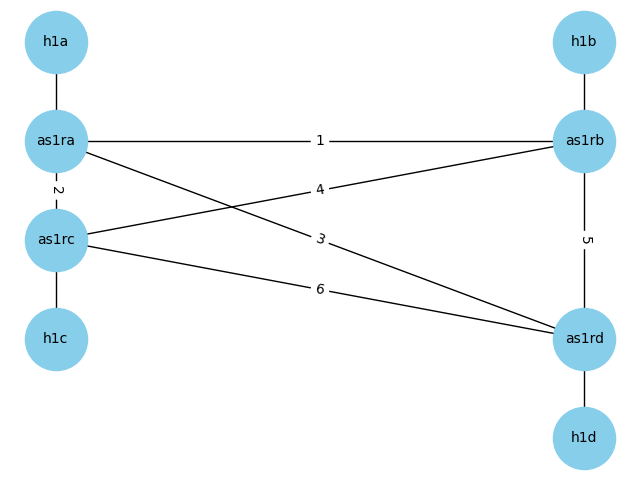
\includegraphics{Lab4/graphics/ospf_topology.png}

\begin{table}[h!]
\centering
\begin{tabular}{|c|c|c|}
\hline
\textbf{Router} & \textbf{Interface Name} & \textbf{IP Address} \\
\hline
as1ra & as1ra-as1rb & fc00:0:1:ab::a/64 \\
\hline
as1ra & as1ra-as1rc & fc00:0:1:ac::a/64 \\
\hline
as1ra & as1ra-as1rd & fc00:0:1:ad::a/64 \\
\hline
as1ra & as1ra-h1a & fc00:0:1:a::a/64 \\
\hline
as1rb & as1rb-as1ra & fc00:0:1:ab::b/64 \\
\hline
as1rb & as1rb-as1rc & fc00:0:1:bc::b/64 \\
\hline
as1rb & as1rb-as1rd & fc00:0:1:bd::b/64 \\
\hline
as1rb & as1rb-h1b & fc00:0:1:b::b/64 \\
\hline
as1rc & as1rc-as1ra & fc00:0:1:ac::c/64 \\
\hline
as1rc & as1rc-as1rb & fc00:0:1:bc::c/64 \\
\hline
as1rc & as1rc-as1rd & fc00:0:1:cd::c/64 \\
\hline
as1rc & as1rc-h1c & fc00:0:1:c::c/64 \\
\hline
as1rd & as1rd-as1ra & fc00:0:1:ad::d/64 \\
\hline
as1rd & as1rd-as1rb & fc00:0:1:bd::d/64 \\
\hline
as1rd & as1rd-as1rc & fc00:0:1:cd::d/64 \\
\hline
as1rd & as1rd-h1d & fc00:0:1:d::d/64 \\
\hline
\end{tabular}
\caption{Interface names and IP addresses sorted by router type}
\label{table:sorted_interfaces}
\end{table}
